\documentclass[11pt,answers]{exam}

% Load useful packages
% Read in necessary packages
\usepackage{import}
\usepackage{amsmath}
\usepackage{amsfonts}
\usepackage{amssymb}
\usepackage{graphicx}
\usepackage{hyperref}
\usepackage{color}
\usepackage{subfigure}
\usepackage{tikz}

% Set various options for exam package
\shadedsolutions % defines the style of the solution environment

% Set lesson name, etc.
\newcommand{\coursename}{Math 312}
\newcommand{\lessonname}{Problem Set 2}
\newcommand{\duedate}{9 February 2016}
\newcommand{\names}{Ian Gallmeister, Kevin Fortune, Alex Webb}

% Set headers/footers to look nice
\pagestyle{headandfoot}
\firstpageheader{\textbf{\large \coursename\ \lessonname}}{}{\textbf{\large Due \duedate}}
\firstpageheadrule
\runningheader{\textbf{\large \coursename\ \lessonname}}{}{\textbf{\large Due \duedate}}
\runningheadrule
\firstpagefooter{\names}{}{Page \thepage\ of \numpages}
\firstpagefootrule
\runningfooter{\names}{}{Page \thepage\ of \numpages}
\runningfootrule

% Define commands related to marking up content
\newcommand{\source}[1]{}

% Define commands related to general mathematical style
\renewcommand{\exp}[1]{e^{#1}}

\renewcommand{\theenumi}{(\alph{enumi})}
\renewcommand{\labelenumi}{\theenumi}
\renewcommand{\thequestion}{\arabic{question}}
\renewcommand{\questionlabel}{(\thequestion)}
%%%%%%%%%%%%%%%%%%%%%%%%%%%%%%%%%%%%%%%%%%%%%%%%%%%%%%%%%%%%

\begin{document}
\begin{questions}

\addtocounter{question}{22}

\item For $\dot{x} = \sin{x}$
\newline\textsc{(a)} Find all fixed points of the flow.
\newline\textsc{(b)} At which points does the flow have the greatest velocity to the right?
\newline\textsc{(c)} \textrm{I} Find the flow's acceleration $\ddot{x}$ as a function of $x$.
\newline \hspace*{1.1em} \textrm{II} Find the points where the flow has the maximum positive acceleration.

\begin{solution}
\newline\textsc{(a)} The fixed points are $x = \{z\pi | z \in \mathbb{Z}\}$
\newline\newline\textsc{(b)} The unstable points are $x = \{(2z + 1)\pi | z\in \mathbb{Z}\}$
\newline\newline\textsc{(c)} \textrm{I} \hspace{3em} $\displaystyle \frac{\partial}{\partial{x}}\left(\dot{x} = \sin{x} \right) \Rightarrow \ddot{x} = \cos{x}$
\newline \hspace*{1.1em} \textrm{II} \hspace{3em} Maximum acceleration at maxima for $\ddot{x}$.  $\ddot{x}_{\hbox{max}} = \{2z\pi | z \in \mathbb{Z}\}$
\end{solution}


\item There are two ways to solve the logistic equation $\dot{N} = rN(1 - N/K)$ analytically for the arbitrary initial condition $N_0$.
\newline\textsc{(a)} Separate variables and integrate using partial fractions.
\newline\textsc{(b)} Make the change of variables $x = 1/N$.  Then derive and solve the resulting differential equation for $x$.

\begin{solution}
\newline\textsc{(a)} - Note, $C$ ignores changes in sign and value since it remains a constant which can be determined later.
\begin{align*}
\frac{\partial{N}}{\partial{t}} &= rN\left(1 - \frac{N}{k}\right) \\
\partial{t} &= \frac{\partial{N}}{rN\left(1 - \frac{N}{k}\right)} \\
\partial{t} &= \partial{N}\left( rN\left(1 - \frac{N}{k}\right) \right)^{-1} = \partial{N}\left(rN - \frac{rN^2}{k}\right)^{-1} \\
\partial{t} &= \partial{N}\left( \frac{k}{rN(k-N)} \right) \\
\\
\frac{k}{rN(k-N)} &= \frac{A}{rN} + \frac{B}{k-N} \Rightarrow A(k-N) + B(rN) = k \\
Ak = k, ~ BrN &= AN \Rightarrow A = 1, ~ B = \frac{1}{r} \\
\int\partial{t} &= \int\partial{N}\frac{1}{rN} + \int\partial{N}\frac{1}{r(N-k)}\\
t + C &= \frac{1}{r}\ln{N} + \frac{-1}{r}\ln(k-N) \\
tr + C &= \ln{N} - \ln(k-N) = \ln{\left( \frac{N}{k-N} \right)} \\
\end{align*}
\begin{align*}
\frac{N}{k-N} &= Ce^{tr} \\
\frac{k-N}{N} &= Ce^{-tr} \\
\frac{k}{N} &= Ce^{-tr} + 1 \\
N &= \frac{k}{C/e^{tr} + 1} = \frac{ke^{tr}}{C + e^{tr}} \\
\end{align*}

\vspace{1em}

\textsc{(b)} - Note - the constants' signs and values will change again to reflect the simplest form in the final solution. (i.e. $k/C$ is also a constant, and will be turned into a new $C$).  For this part, we use the chain rule and substitution to get an equation for $\partial{x}/\partial{t}$, use separation of variables, and solve.  Towards the end, we invert it and manipulate our result to get the same result as the prior part of the problem.
\begin{align*}
\frac{\partial{x}}{\partial{t}} &= \frac{\partial{x}}{\partial{N}}\cdot\frac{\partial{N}}{\partial{t}} \\
x = \frac{1}{N} &\Rightarrow \frac{\partial{x}}{\partial{N}} = \frac{-1}{N^2} = -x^2\\
\frac{\partial{N}}{\partial{t}} &= rN\left(1 - \frac{N}{k}\right) = \frac{r}{x}\left( 1 - \frac{k}{x} \right)
\frac{\partial{x}}{\partial{t}} = \frac{\partial{x}}{\partial{N}}\frac{\partial{N}}{\partial{t}} = \left(-x^2\right)\left(\frac{r}{x}\left( 1 - \frac{1}{kx}\right)\right) \\
&= -rx \left(1 - \frac{1}{kx}\right) \\
\partial{t} &= \frac{\partial{x}}{-rx \left(1 - \frac{1}{kx}\right)} \\
t + k &= \frac{-1}{r}\ln{\left( \frac{r}{k} - rx \right)} \hbox{ and exponentiate to get} \\
\frac{r}{k} - rx &= Ce^{-tr} \\
rx &= \frac{1}{r}\left( \frac{r}{k} - \frac{1}{Ce^{tr}} \right)\\
x &= \frac{kCe^{tr}}{kCe^{tr}}\left( \frac{1}{k} - \frac{1}{Ce^{tr}} \right)  \\
x &= \frac{Ce^{tr} - k}{kCe^{tr}} \\
x = \frac{1}{N} &\Rightarrow N = \frac{1}{x} = \frac{kCe^{tr}}{Ce^{tr} - k} = \frac{C(ke^{tr})}{C(e^{tr} - k/C)} \\
N &= \frac{ke^{tr}}{e^{tr} - C}
\end{align*}
\end{solution}

\item The growth of cancerous tumors can be modeled by the Gompertz Law $\dot{N} = -aN\ln{(bN)}$ where $N(t)$ is proportional to the number of tumor cells and $a, b > 0$ are parameters.
\newline\textsc{(a)} Interpret $a$ and $b$ biologically.
\newline\textsc{(b)} Sketch the vector field and graph $N(t)$ for various initial values.

\begin{solution}
\newline\textsc{(a)} $a$ is a growth factor for exponential growth.  $b$ is a growth factor if greater than or equal to $1$.  Otherwise it'll limit growth as $bN$ goes to $1$
\newline\newline\textsc{(b)}

This graph shows the change in N(t) over t with various initial conditions. 

\begin{center}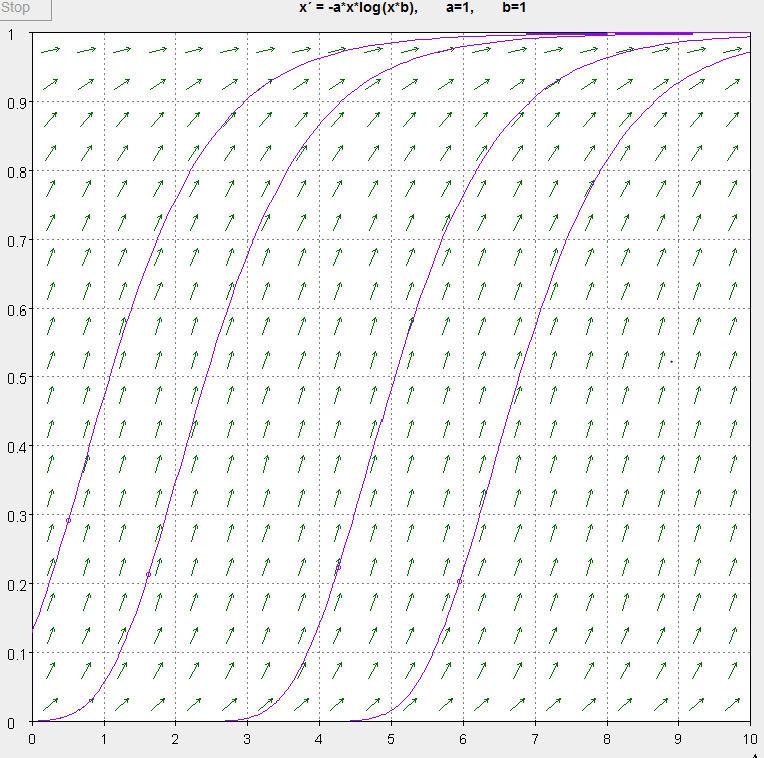
\includegraphics[width = 0.45\textwidth]{sketch}\end{center}
\end{solution}

\item Dominance of the fittest.  Suppose $X$ and $Y$ are two species that reproduce exponentially fast: $\dot{X} = aX$ and $\dot{Y} = bY$, respectively, with initial conditions $X_0, Y_0 > 0$, and growth rates $a > b > 0$. Here $X$ is “fitter” than $Y$ in the sense that it reproduces faster, as reflected by the inequality $a > b$. So we’d expect $X$ to keep increasing its share of the total population $X + Y$ as $t \to \infty$ . The goal of this exercise is to demonstrate this intuitive result, first analytically and then geometrically.
\newline\textsc{(a)} Let $x(t) = X(t)/[X(t) + Y(t)]$ denote $X$'s total share of the population.  Solve for $X(t)$ and $Y(t)$ to show that $x(t)$ increases monotonically and approaches $1$ as $t$ goes to $\infty$.

\begin{solution}

We can solve $\dot{X}$ and $\dot{Y}$ via separation of variables.

$$\frac{dx}{X} = dt*a$$ $$\frac{dY}{Y} = dt*b$$

$$ln(X) = at + C_1$$ $$ln(Y) = bt + C_2$$

$$X = \exp{at+C1}$$ $$Y = \exp{bt+C_2}$$

$$X = C_3\exp{at}$$ $$Y = C_4\exp{bt}$$

Given the initial conditions, we can solve for the constants $C_3$ and $C_4$:

$$ X = X_{0}\exp{at}$$ $$ Y = Y_{0}\exp{bt}$$

Solve for Y(t) and X(t) in x(t) to find the function x(t) in terms of t:

$$x(t) = \frac{X(t)}{X(t) + Y(t)}$$

$$x(t) = \frac{X_{0}\exp{at}}{X_{0}\exp{at} + Y_{0}\exp{bt}}$$

As t approaches infinity, the $\exp{bt}$ term becomes insignificant because a $>$ b. Therefore, we can rewrite the equation as 

$$x(t) = \frac{X_{0}\exp{at}}{X_{0}\exp{at}} = 1$$

We know that the function is monotonic because:

$$\dot{x} = \frac{(X_{0}Y_{0}(a-b)e^{(a+b)t}}{(X_{0}e^{at}+Y_{0}e^{bt})^2}$$

$\dot{x}$ is always positive because a $>$ b. 

\end{solution}

\textsc{(b)} Alternatively, we can arrive at the same conclusions by deriving a differential equation for $x(t)$. To do so, take the time derivative of $x(t) = X(t)/[X(t) + Y(t)]$ using the quotient and chain rules. Then substitute for $\dot{X}$ and $\dot{Y}$ and thereby show that $x(t)$ obeys the logistic equation $\dot{x} = (a-b)x(1-x)$.  Explain why this implies that $x(t)$ increases monotonically and approaches $1$ as $t \to \infty$.

\begin{solution}

$$x(t) = \frac{X(t)}{X(t) + Y(t)}$$

$$\dot{x}(t) = \frac{[X(t) + Y(t)]\dot{X}(t) - X(t)[\dot{X}(t) + \dot{Y}(t)]}{[X(t) + Y(t)]^2}$$

We have functions of $\dot{X}$ and $\dot{Y}$ which we can substitute into the above equation:

$$\dot{x}(t) = \frac{[X(t) + Y(t)][a*X(t)] - X(t)[a*X(t) + bY(t)]}{[X(t) + Y(t)]^2}$$

$$ = \frac{aX}{X+Y} - \frac{X(aX+bY)}{(X+Y)(X+Y)}$$

$$ = ax - x\frac{aX+bY}{X+Y}$$

$$ = ax - x(ax+b(1-x))$$

$$ = ax - ax^2 - bx(1-x)$$

$$ = x(a-ax-b(1-x))$$

$$ = x(a(1-x)-b(1-x)$$

$$ \dot{x}= x(a-b)(1-x)$$

That is the form of the logistic equation. This implies that x is monotonic because a $>$ b, so the quantity is always positive. This also implies that x is 1 as t approaches infinity because $\dot{x}$ is 0 as x approaches 1. In other words, there is a stable fixed point at x = 1.

\end{solution}

\item In statistical mechanics, the phenomenon of ``critical slowing down" is a signature of second-order phase transition.  At the transition, the system relaxes to equilibrium much slower than normal.  Here's a mathematical version:
\newline\textsc{(a)} Obtain the analytical solution for $\dot{x} = -x^3$ for an arbitrary initial condition $x_0$.  Show that $x(t) \to 0$ as $t \to \infty$ but that the decay is not exponential. (It should be a much slower algebraic function of $t$)
\newline\textsc{(b)} To get some information about the slowness of decay, create a plot for the solution given the initial condition $x_0 = 10$ for $0 \leq t \leq 10$.  On the same graph, also plot the solution to $\dot{x} = -x, ~ x_0 = 10$. 

\begin{solution}
(A)
\begin{equation*}
\frac{dx}{dt} = -x^3
\end{equation*}
\begin{equation*}
-x^{-3} dx = dt
\end{equation*}
Take the integral of both sides to obtain:
\begin{equation*}
\frac{-x^{-2}}{2} = t + C
\end{equation*}
\begin{equation*}
\frac{1}{x^2} = t + C
\end{equation*}
\begin{equation*}
x = \sqrt{\frac{1}{2t + C}}
\end{equation*}
Let the arbitrary initial condition be $x(0) = x_0 = 0$. So 
\begin{equation*}
x_0 = \sqrt{\frac{1}{C}}
\end{equation*}
\begin{equation*}
C = x_0 ^{-2}
\end{equation*}
Finally, we have the solution
\begin{equation*}
x = \sqrt{\frac{1}{2t + x_0 ^{-2}}}
\end{equation*}
As t gets larger, $2t + x_0 ^{-2}$ also gets larger, so $\sqrt{\frac{1}{2t + x_0 ^{-2}}}$ gets very small. Therefore, as $t \to \infty$, x approaches $0$. \\ 
\newline\newline\textsc{(b)} 
\begin{equation*}
\frac{dx}{dt} = -x
\end{equation*}
\begin{equation*}
\frac{dx}{x} = dt
\end{equation*}
Take the integral of both sides to obtain:
\begin{equation*}
-\ln(x) = t+ C
\end{equation*}
\begin{equation*}
x = -Ce^t
\end{equation*}
Given $x_0 = 10$,
\begin{equation*}
x = -10e^t
\end{equation*}

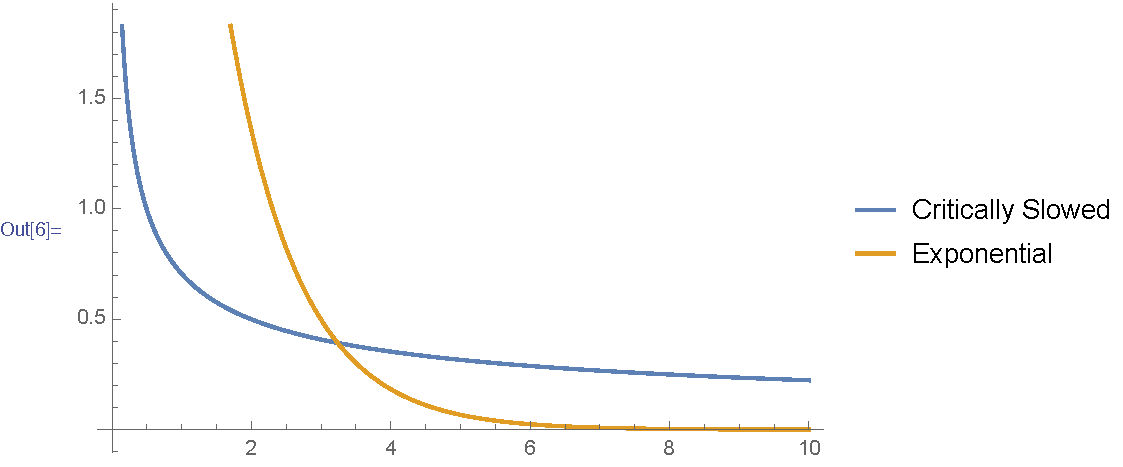
\includegraphics[width = \textwidth]{plot}
\end{solution}

\item A particle travels on the half-line $x \geq 0$ with a velocity given by $\dot{x} = -x^c, ~ \hbox{ constant } c \in \mathbb{R}$.
\newline\textsc{(a)} Find all values of $c$ such that the origin $x = 0$ is a stable fixed point. 
\newline\textsc{(b)} Now assume that $c$ is chosen such that $x = 0$ is stable. Can the particle ever reach the origin in a
finite time? Specifically, how long does it take for the particle to travel from $x = 1$ to $x = 0$, as a
function of $c$?

\begin{solution}
\newline\textsc{(a)} There are three cases for $c$: $c > 0, c < 0, c = 0$.
\newline If $c > 0$, then the function is negative with a value approaching zero as $x^+ \to 0$.  This works.
\newline If $c = 0$, the derivative is -1 which has no fixed points, stable or unstable, anywhere.  This doesn't work.
\newline If $c < 0$, the derivative is $\frac{1}{x^c}$, a function that goes to $\pm\infty$ at $x=0$ which doesn't beget a stable fixed point.
\newline Thus, there is a stable fixed point at $x=0$ for all $c \in \mathbb{R}> 0$
\newline\newline\textsc{(b)} It helps to solve this problem first:
\begin{align*}
\frac{\partial{x}}{\partial{t}} &= -x^c \\
\int \frac{\partial{x}}{x^c} &= -\int\partial{t} \\
\frac{x^{1-c}}{1-c} &= -t + k \\
t &= \frac{x^{1-c}}{c-1} + k \\
\end{align*}
At $x =0$, $t = k$.  At $x = 1$, $t = k + \frac{1}{c-1}$.  Therefore, the time it takes to travel from $x = 1$ to $x = 0$ is $\Delta t = t_0 - t_1 = k - \left( k + \frac{1}{c-1} \right) = -\frac{1}{c-1} = \frac{1}{1-c}$.  This time exists and is positive for $c < 1$.  At $c = 1$, $\Delta t$ is undefined, and at $c > 1$ it is negative.  It is not possible for a particle to take negative time going from one place to another, so the particle only makes it from $x = 1$ to $x = 0$ in a finite time if $ c < 1$
\end{solution}

\item Consider the equation $\dot{x} = rx + x^3$, where $r > 0$ is fixed. Show that $x(t) \to \pm\infty$ in finite time,
starting from any initial condition $x_0 \neq 0$.

\begin{solution}
For $x_0 > 0$, $\dot{x} > 0$ which implies that the function is increasing.  A little farther along, $x_1 > x_0$ so $\dot{x}$ is larger and the function increases.  This continues off to $\infty$ getting faster and faster all the time.
\newline For $x_0 < 0$, $\dot{x} < 0$, and the derivative's magnitude will only increase (since $rx$ and $x^3$ always have the same sign), sending $x$ to $-\infty$
\end{solution}

\end{questions}
\end{document}